\subsubsection{Using C++ API}
\label{sec:tracing_cpp_api}

The KisTA library enables the creation of a VCD trace of the utilizations of the tasks assigned to each scheduler.
%
Listing~\ref{list:trace_rtos_activity} shows the API for controlling tracing tasks and scheduler activity.

%\begin{table}[t]
\begin{lstlisting}[style=KistaCodeStyle,caption={API for controling tracing tasks and scheduler activity.},label=list:trace_rtos_activity]
class scheduler : public sc_module {
...
public:
   ...
   void trace_utilizations(std::string &scheduler_trace_file_name_par);
   void trace_utilizations();
   ...
};
\end{lstlisting}
%\end{table}

The KisTA model only has to call the \texttt{trace\_utilizations()} method associated to an scheduler.
%
When this method is called (it has to be done before the simulation start), the scheduler object generates a trace file at the end of the simulation.
%
Therefore, a scheduler file is generated for each scheduler instance. 

Assuming that the name of the scheduler instance is of the type \texttt{<sched\_name>},
the name of the trace file will be \texttt{<sched\_name>\_trace.vcd} on the default.
The user can set the name of the trace file by providing a name parameter (the method \texttt{trace\_utilizations(std::string file\_name)} is used then).

The .vcd file can be plotted with any VCD compatible viewer (e.g. \emph{gtkwave}).
Figure~\ref{fig:trace_example} shows an example where the trace of 4 tasks statically scheduled on
a scheduler called \emph{sched1} has been visualized with \emph{gtkwave}.
In such an example, the scheduler has been configured to use an scheduling penalty of 0s.

\begin{figure}[h]
\centering
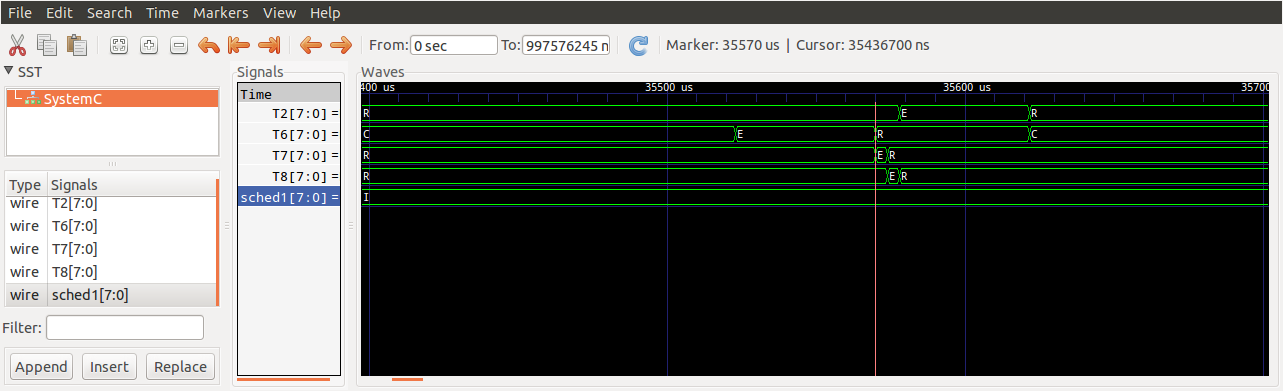
\includegraphics[width=\textwidth]{./figs/trace_sched1_static_sched.png} 
\label{fig:trace_example}
\caption{A gtkwave visualization of tasks and scheduler activity reported by KisTA} 
\end{figure}

\subsubsection{Using the XML front-end}
\label{sec:tracing_xml}

The KisTA-XML front-end enables to configure the tracing of the scheduler activity.
%
For it, the \texttt{trace\_rtos} tag within the analysis section is used.
The \texttt{trace\_rtos} tag has associated a mandatory attribute \texttt{name} which shall contain the name of the scheduler instance which the tracing is done for.
%
Therefore, the generation of trace files is specified for each scheduler.
%
If no more attributes are provided, the name of the VCD file generated follows simular rules as was explained in Section~\ref{sec:tracing_cpp_api}.
%
The XML interface also allows to specify the name of the trace file by means of the \texttt{file} attribute, associated to to the \texttt{rtos\_trace} entry.

%\begin{table}[t]
\begin{lstlisting}[language=XML, caption={Setting tracing from the XML interface.}, label=list:xml_trace_setting]
<kista_configuration>
   ...
   <analysis>
      <rtos_trace name="sched1"/>
      <!-- Trace RTOS activity -->
      <!-- A trace file called sched1_trace.vcd will be generated -->
      <rtos_trace name="sched2" file="rtos2_trace"/>
      <!-- Trace RTOS activity -->
      <!-- A trace file called rtos2_trace.vcd will be generated -->
      ...
   </analysis>
   ...
</kista_configuration>
\end{lstlisting}
%\end{table}



